\chapter{Az ókeresztény és a bizánci művészet} % Introduction
\label{ch:4_okereszteny_bizanc}

\section{Az ókeresztény és a bizánci építészet, festészet és díszítőművészet}

\tcbox[left=0mm,right=0mm,top=0mm,bottom=0mm,boxsep=0mm,
toptitle=0.5mm,bottomtitle=0.5mm,title=\centering{A tétel adatai}]{%
	
	\begin{tabular}{| p{0.25\textwidth} | p{0.7\textwidth} |}
		
		\hline
		Tétel teljes címe
		&
		Mutassa be az ókeresztény és a bizánci művészetet - az építészet és a festészet, valamint a díszítőművészet stílusjegyeit, ismert alkotásait!
		\\ \hline
		
		Jegyzetek
		&
		\begin{compactitem}
			\item Az ókeresztény és bizánci építészet - a bazilika és a bizánci templom felépítése.
			\item Az ókeresztény szobrászat stílusjegyei és jelképei.
			\item A bizánci mozaik, az ikonfestészet és a kézművesség jellemzői.
		\end{compactitem}
		\\\hline
		
	\end{tabular}}

\subsection*{Történelmi háttér}

\subsubsection{A Római Birodalom ketté válik}
A Római Birodalom a Kr.u. V.sz.-ban ketté válik: Nyugat-Római és Kelet-Római Birodalommá. Kr.u. 476-ban a népvándorlás, az Európát elárasztó barbár népek betöréseinek következtében a Nyugat-Római Birodalom megbukik, míg a keleti rész Bizánc néven fejlődésnek indul.

\subsubsection{Nyugat-Római Birodalom - Ókeresztény művészet}

Az Ókeresztény művészet színtere a Nyugat-Római Birodalom területe volt. A korszak a legelső keresztény közösségek létrejöttétől (Kr.u. 40-es évek) a Nyugat-Római Birodalom bukásáig (Kr.u. 476) tartott.

\paragraph{Két korszaka}
Az ókeresztény művészet a 313-as évszám két részre osztja.

\subparagraph{Üldözött korakereszténység}
A milánói ediktum (313-ig) előtti ókeresztény művészet. A keresztény vallás államvallássá tételéig tartó korszak, amelynek nem lehetett hivatalos, szabadon alkalmazható művészete, nem épülhettek templomok, stb., ezért ebben az időben rejtett helyeken, rejtett témájú műalkotások készültek.

\subparagraph{A milánói ediktum}
Kr. u. 313.: Nagy Konstantin kiadja a „milánói ediktumot”. Ebben a rendeletben engedélyezi a keresztény vallás gyakorlását, és visszaadja az egyház vagyonát, majd törvényrendeletet hoz a keresztényüldözések betiltására.

\subparagraph{A milánói ediktum (313) utáni ókeresztény művészet}
z utolsó római egyben első keresztény császárok kora vagy késő-római művészet. Nagy Konstantin császár és Nagy Theodóziusz császár és utódaik kora ez, amikor az egyház állami, császári támogatást kapott építkezéseihez, így hatalmas templomok monumentális mozaikokkal épültek.

\subsubsection{Kelet-Római Birodalom területén - Bizánci művészet}
A Bizánci birodalom a kelet-római birodalom területén (mai Görög- és Törökország), a nyugati római birodalom bukása (Kr. u. 476) után kialakuló birodalom, amely Konstantinápoly, vagy más néven Bizánc (ma Isztambul) irányításával egészen a 15. századig él. A 11.sz-tól az ortodox keresztény vallás az uralkodó a területén.

\subsection*{Hitvilág}

A keresztény vallás, a keresztény Biblia. A keresztény vallás a zsidó hitvilágból ered.

\paragraph{Ószövetség}
A zsidó nép történetét beszéli el az ember teremtésétől a rómaiak koráig. Ezek a szövegek a mai tudomány szerint is már a kereszténység megszületése előtt léteztek. Az ószövetség prófétáinak könyvei gyakran jövendölnek egy Messiásról, aki a történelme során számtalanszor leigázott, meghurcolt kiválasztott népet megszabadítja a szenvedéstől, és feléleszti, visszaállítja annak dicsőségét. Az első – zsidókból lett - keresztények Jézusban találták meg ezt a Messiást.

\paragraph{Újszövetség}
Jézus életét (majd az apostolok térítő tevékenységét) beszéli el. Ezeknek a szövegeknek a születését a mai tudomány a Kr.u. 1.sz. végére teszi. A szövegek (evangéliumok) Jézus tevékenysége mellett arról is beszámolnak, hogy Jézus feltámadt a halála után. Ez a keresztény vallás alapja, erre alapozva tartják a keresztények Jézust nem pusztán prófétának, hanem Isten Fiának, egyszerre isteni és emberi természettel rendelkezőnek, és abban hisznek, hogy maga az Isten – akit azonosnak tartanak a zsidó nép istenével, akit az Ószövetség Jahvénak nevez, az Újszövetség pedig Atyának – Jézus személyében, emberi alakot öltve megjelent a földön.

\subsection*{Az ókeresztény művészet}

\subsubsection{Építészet}

	\paragraph{Gyülekezeti házak}
	Gyülekezeti hellyé, szertartáshellyé alakított magánház – az üldözések miatt a korai keresztény kis közösségeknek nem volt hivatalos gyülekező helyük, ahol szertartásaikat tarthatták volna, ezért erre a célra magánházaikat alakították át.
	
	Például a szokványos átriumos római lakóház lakóhelyiségeiből keresztelő medencés kápolnát és körpados gyülekezeti termet alakítottak ki.
	
	\subparagraph{Agapé:} (jelentése szeretetlakoma) a gyülekezeti házakban a korai keresztény közösségek kötetlen szertartásra, istentiszteletre jöttek össze, melyben az utolsó vacsorára emlékeztek kenyértöréssel.
	
	\begin{wrapfigure}{r}{0.45\textwidth}
		\tcbox[colback=darkgray!85!black,
		left=0mm,right=0mm,top=0mm,bottom=0mm,boxsep=1mm,toptitle=0.5mm,bottomtitle=0.5mm,
		title=\centering{Katakomba, Róma}]{
			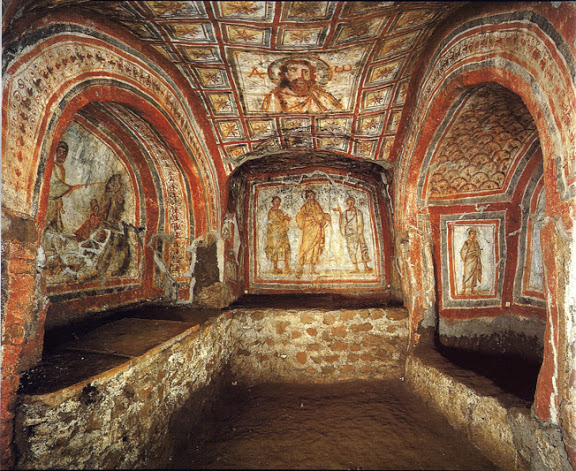
\includegraphics[width=1.0\linewidth]{04/katakomba}
		}
	\end{wrapfigure}
	
	\paragraph{Katakombák}
	A korai keresztény közösségek földalatti temetkezőhelyei (a szó jelentése: „kata” = -nál, -nél; „kümbé” = verem $\rightarrow$ „a veremnél”).
	
	Főleg Rómában találhatóak. Szűk (1m széles, 3-4 m magas), hosszú folyosók hálózata. A falakban téglalap alakú vagy íves kialakítású, márványlapokkal lezárt sírhelyek vannak
	
		\subparagraph{Katakombákba temetkezés okai}
		Egész testes temetkezés (a test feltámadásába vetett hit miatt).
		
		Vértanútisztelet: tisztelték mindazokat, akik az üldözésekben hitükért föláldozták az életüket, és a katakombákba temették őket, hogy szabadon látogathassák a sírjaikat.
		
		A vértanúk sírhelyét gazdagabban kiépítették, itt a folyosó kiszélesedik, falait falfestményekkel díszítették; itt gyakran összegyűltek és szertartásokat tartottak; az ilyen gazdagabban díszített vértanú-sírhelyeket cubiculum-nak [kubíkulum] nevezzük.
	
		\subparagraph{Katakombafestészet}
		
		Stílusuk nem új, a római festészettől nem tér el, nagy fehér felületeken táblaképeket imitáló betétképek vannak = ált. vörös keretben jelenik meg egy kevés alakos kompozíció; a vörös, az okkersárga, a zöld a leggyakoribb szín
		
		Témáik mindig keresztény tartalmúak, a katakombaképek jelentősége, hogy a következő évszázadok keresztény témái ekkor, a katakombákban alakulnak ki. Négy csoportba sorolhatók:
		\begin{compactitem}
			\item  ószövetségi és újszövetségi események ábrázolása,
			\item eredetileg római vagy görög mitológiai téma keresztény tartalommal, pl. \textit{Jó Pásztor} (Jézus, aki népét, mint nyájat terel), 
			\item szimbólumok (hal ~ Jézus, XP ~ Krisztus-monogram),
			\item az ókeresztény közösségek életeseményeinek ábrázolása (\textit{Orans alak} ~ kezeit széttárva imátkozó alak, \textit{Agapé} ~ szeretetlakoma ábrázolása).
		\end{compactitem}
	
	\paragraph{Templomépítészet}
	
		\subparagraph{Longitudinális templomok}
		Hosszanti elrendezésű templom. Célja a nagyszámú hívő tömeg befogadása - a keresztény templomnak, térnek tükröznie kell azt, hogy a keresztény hitben vállalt világ elkülönül a mindennapitól, a hívőnek el kell zárkóznia a külső világtól, amikor a hitével foglalkozik (az antik templomokba nem mehettek be a hívők).
		\begin{itemize}
			\item Ókeresztény bazilikák
			\begin{compactitem}
				\item Alaprajzuk, felépítésük eredete: a római kori bazilikát vették mintául, hiszen ez az épülettípus tudott sok embert befogadni.
				\item a bejáratot áthelyezik a rövidebbik oldalra, így a hosszúkás elrendezés új szimbolikus értelmet kap: a keresztény hívő útja a bejárattól az oltárig („szent út”) = út az evilági életből a szent élet felé.
				\item A fő különbség a római kori és az ókeresztény bazilika között az, hogy a római bazilika középület volt, az ókeresztény bazilika viszont templom.
			\end{compactitem}
			
			\item A Régi Szent Péter Bazilika, Róma
			\begin{compactitem}
				\item Nagy Konstantin kezdi építtetni Kr.u. 333-ban Szent Péter sírja fölött, több mint 100 évig folyik az építkezés.
				\item Az egyház legfontosabb temploma volt, de már nem áll, csak feltárásokból ismerjük az alaprajzát, fennmaradt rajzokból a külsejét és egy freskóból a belsőt; mert a XVI-XVII. sz-ban egy jóval nagyobb barokk templomot építettek a helyére.
			\end{compactitem}
		
			\item A bazilika térszerkezete, elemei
			\begin{compactitem}
				\item Alaprajza longitudinális elrendezésű – az egész egy térsor, ahol a terek a szentély felé haladva egyre kevesebb hívőt fogadnak be és egyre szentebb funkciót töltenek be – épp, mint az egyiptomi templomoknál. (Egyiptom területén terjedt el a kereszténység legkorábban.)
				
				\item Öthajós, hajó: a hívek befogadására szolgáló hatalmas, osztatlan térrész, azaz csarnok, a „szent út” helye. A belső tér nagyságát a hajók számának növelésével lehetett fokozni.
				
				\item Bejáratuk a rövidebbik oldalon van.
				
				\item Átrium = a bejárat előtt lévő négyzet alaprajzú, nyitott tetejű előudvar, melyet oszlopos folyosók vesznek körbe, középen általában keresztelőkút, keresztelő-medence van – itt keresztelték meg a hívőket. Nevét a római lakóházak hasonlóan nyitott udvaráról kapta.
				
				\item Narthex = (tornác) az átrium és a hosszház közötti, a templom teljes szélességében húzódó, nyújtott téglalap alakú előcsarnok, ami a görög és római templomok előcsarnokához hasonló térrész; célja a szent épületre való ráhangolódás; itt tartózkodhattak a még meg nem kereszteltek.
				
				\item Kereszthajó = a hosszhajók és az apszis között keresztirányba futó hajó a nagyszámú papság és a kórus számára; magassága azonos a főhajóéval.
				
				\item Apszis: A bejárattal szemben, a vértanú sírja fölött az ún. apszis = félköríves szentély található, itt tartózkodott a papság (a félköríves térrész már a császárkori római kori bazilikákban is megjelent, itt volt a császár trónusa vagy szobra, az ókeresztény bazilikákban ennek helyére a püspöki trónus kerül).
				
				\item Négyezeti tér / Kórus = nevét az apszis előtt a főhajó és a kereszthajó találkozásánál kialakuló négyzet alaprajzáról kapta, itt áll az oltárasztal, az ún. mensa, és a vallásos iratok felolvasását szolgáló emelvények (a gyakran itt tartózkodó énekkarról kórusnak is szokás nevezni).
				
				\item Térlefedés: Ún. gerendázatos nyitott fedélszékkel fedték le a hajókat.
				
				\item Bazilikális szerkezet: az oldalhajók magassága a főhajóéhoz képest alacsonyabb, hogy a főhajó a kiemelkedő falain nyitott ablakokon keresztül megvilágítást kaphasson.	
				
				\item Az ókeresztény templomok külseje jelentéktelen, díszítetlen, mert a hívő tömeg az épületen belül helyezkedik el, így a belső térre kerül a hangsúly.
				
				\item Egyetlen, az épülettől, a homlokzattól külön álló harangtorony = a campanile kapcsolódik hozzá.		
			\end{compactitem}
		\end{itemize}
	
		\begin{figure}[H]
			\centering
			\begin{minipage}{0.4\textwidth}
				\tcbox[colback=darkgray!85!black,
				left=0mm,right=0mm,top=0mm,bottom=0mm,boxsep=1mm,toptitle=0.5mm,bottomtitle=0.5mm,
				title=\centering{A bazilika felépítése}]{
					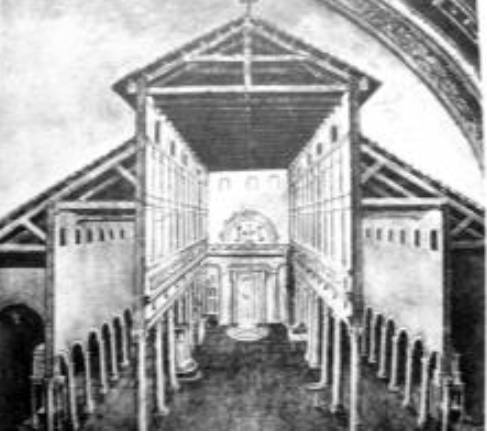
\includegraphics[width=1.0\linewidth]{04/bazilika}
				}
			\end{minipage}
			\hfill
			\begin{minipage}{0.55\textwidth}
				
				\tcbox[colback=darkgray!85!black,
				left=0mm,right=0mm,top=0mm,bottom=0mm,boxsep=1mm,toptitle=0.5mm,bottomtitle=0.5mm,
				title=\centering{A régi Szent Péter bazilika}]{
					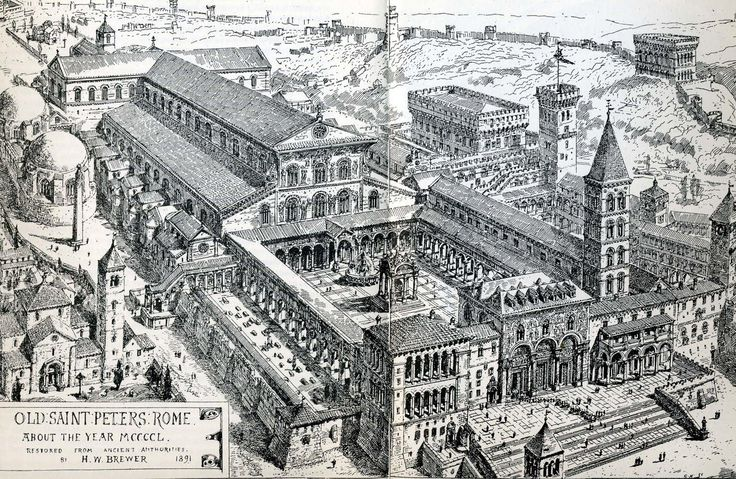
\includegraphics[width=1.0\linewidth]{04/regi_szent_peter_bazilika}
				}
			\end{minipage}
		\end{figure}
		
		\subparagraph{Centrális templomok}
		A centrális = központos elrendezésű (kör, sokszög, görögkereszt /=plusz jel/ alaprajzúak) olyan kisméretű templomok, amik egy tisztelt vértanú sírja fölötti emlékkápolnák vagy keresztelőkápolnák.
		
		Kör, sokszög vagy görögkereszt alakúak, külsejük puritán, belsejük mozaikkal díszített.
		\begin{itemize}
			\item \textbf{Santa Costanza temploma, Róma}: Nagy Konstantin leányának, Konstanzának építteti, az ő sírja fölé emlékkápolnaképpen. Bejárata előtt narthex található. A kupolás tér körül körfolyosó van, ami ún. gyűrűs dongaboltozattal fedett.
		\end{itemize}
		
		 \begin{center}
		 	\tcbox[colback=darkgray!85!black,
		 	left=0mm,right=0mm,top=0mm,bottom=0mm,boxsep=1mm,toptitle=0.5mm,bottomtitle=0.5mm,
		 	title=\centering{Santa Constanza templom, Róma}]{
		 		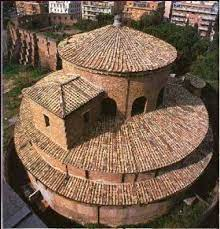
\includegraphics[width=0.33\linewidth]{04/santa_constanza}
		 		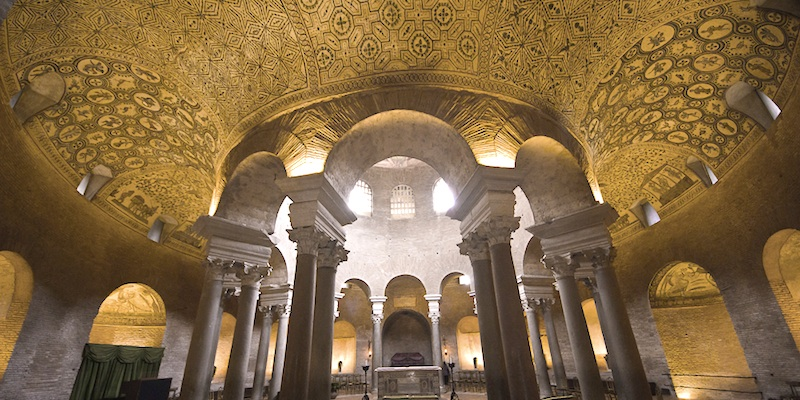
\includegraphics[width=0.65\linewidth]{04/santa_constanza_belseje}		}
		 \end{center}
		
	
		\begin{itemize}
			\item\textbf{Galla Placidia sírtemplom, Ravenna}: Galla Placidia Nagy Teodóziusz császár leánya, az ő sírja fölé épült síremléktemplomnak, Kr. u. 425körül. Alaprajza görögkereszt alakú. Görögkereszt (+): olyan kereszt-forma, melynek szárai azonos hosszúságúak.
		\end{itemize}
	
		\begin{center}
			\tcbox[colback=darkgray!85!black,
			left=0mm,right=0mm,top=0mm,bottom=0mm,boxsep=1mm,toptitle=0.5mm,bottomtitle=0.5mm,
			title=\centering{Galla Placidia sírtemplom, Ravenna}]{
				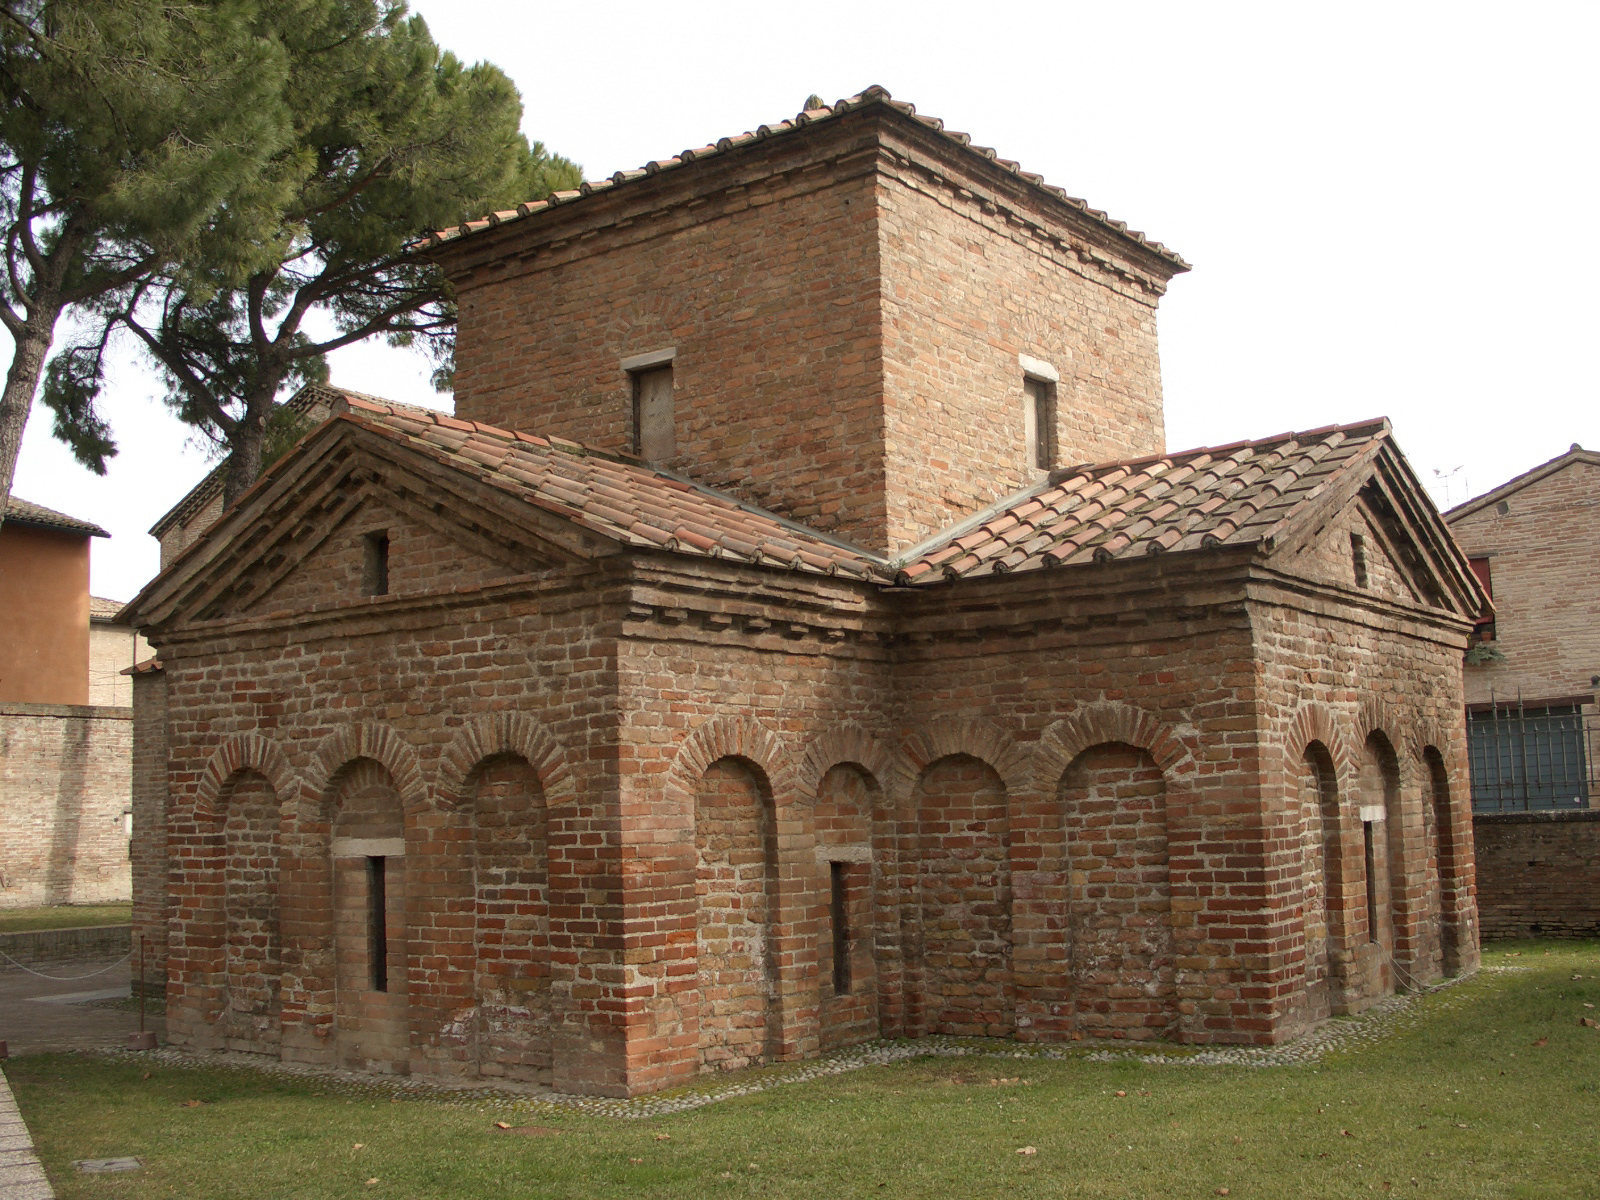
\includegraphics[width=0.42\linewidth]{04/galla_placidia}
				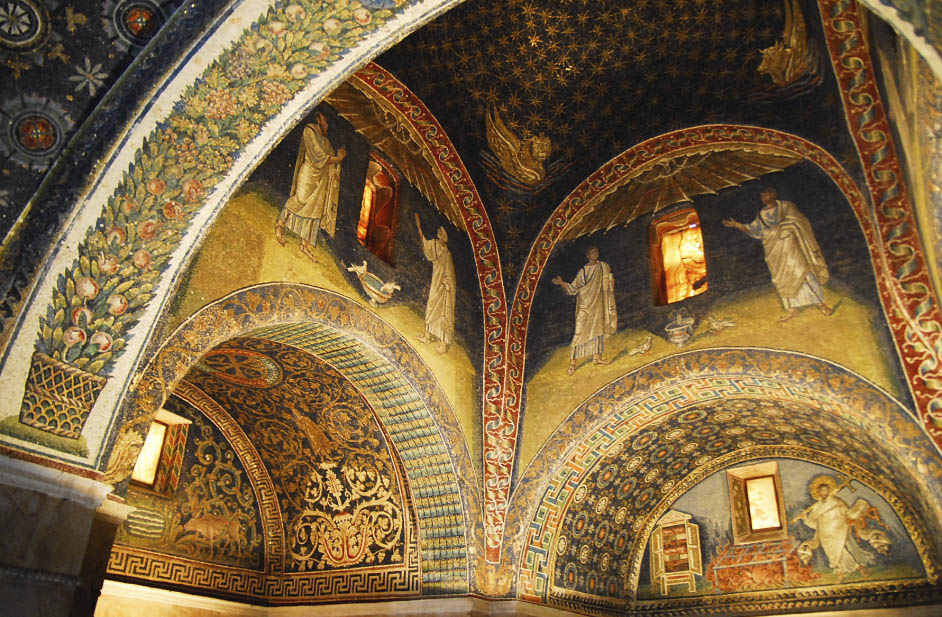
\includegraphics[width=0.48\linewidth]{04/galla_placidia_belseje}
			}
		\end{center}
		
		
\subsubsection{Mozaikművészet}

	Az ókeresztény templomok külseje rendkívül puritán. A belső ezzel ellentétben igen gazdagon díszített. A díszítés leggyakoribb módja a mozaik: apró festett, vagy színes kövekből, kerámiából, üvegdarabokból kialakított kép.
	
	A mozaik már a rómaiak idején is létezett, de míg ott főleg a földön, dekoratív padlóburkolatként kapott helyet, az ókeresztény korban a mozaikok a falra kerülnek.

	\paragraph{Téma}
	Keresztény témájúak, kedvelik a szimbólumokat, de magukon viselik az antikvitás hagyományát is. Így gyakran ábrázolnak olyan motívumot, figurát, ami az antik művészetben is létezett, de ez a motívum itt átértelmezve, keresztény gondolatkörben, keresztény témaként szerepel. (pl.: Jó pásztor, Szőlőindák)
	
	\paragraph{Stílus}
	Nem törekednek a valóság visszaadására, nem reálisak, de a római hagyomány a stílusban sem múlik el nyom nélkül: nincs térábrázolás, ugyanakkor itt-ott mégis feltűnik a perspektíva; a figurák visszafogott mozdulatokat tesznek, de gyakran kontraposztban állnak. Színekben a kék és az arany dominál, ezek is szimbolikusak, nem a valóság visszaadását szolgálják, hanem az égre, a fényre, a téma szent voltára utalnak.
	
	\begin{wrapfigure}{r}{0.45\textwidth}
		\tcbox[colback=darkgray!85!black,
		left=0mm,right=0mm,top=0mm,bottom=0mm,boxsep=1mm,toptitle=0.5mm,bottomtitle=0.5mm,
		title=\centering{Szőlőszedők mozaik, Santa Constanza, Róma}]{
			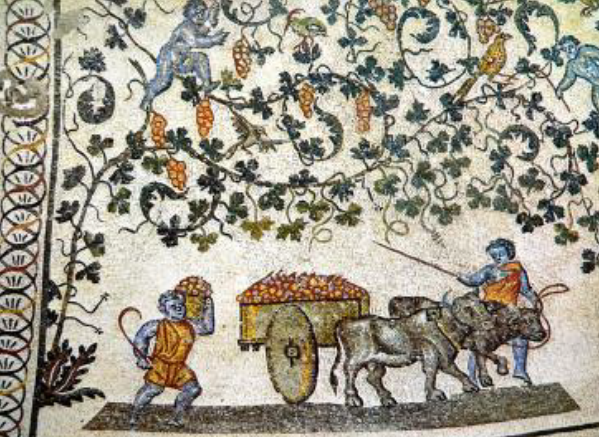
\includegraphics[width=1.0\linewidth]{04/szoloszedok}
		}
		\tcbox[colback=darkgray!85!black,
		left=0mm,right=0mm,top=0mm,bottom=0mm,boxsep=1mm,toptitle=0.5mm,bottomtitle=0.5mm,
		title=\centering{Jó pásztor mozaik, Galla Placidia, Ravenna}]{
			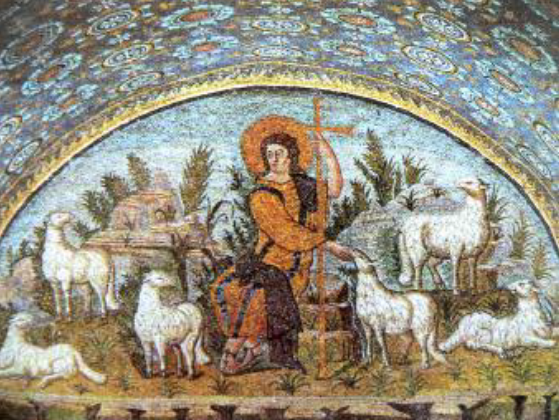
\includegraphics[width=1.0\linewidth]{04/jo_pasztor}
		}
	\end{wrapfigure}
	
	\paragraph{Szőlőszedők}
	A mozaik a Santa Constanza templomban van.
	
	Az antik (görög, római) mozaikokat követi abban, hogy szőnyegszerű: nem történetet mesél el, hanem dekoratív, de a padló helyett a mennyezetre került
	Látszólag kizárólag díszítő jellegű az ábrázolás: puttók szőlőindák közt szőlőfürtöket szednek
	
	Az antikos ábrázolás keresztény tartalmat kap: utalás Jézus példabeszédeire, melyben a szőlőmunkásokat az igaz hit hirdetőivel azonosítja; utalás a borra, amely a keresztény liturgiában Krisztus vére.
	
	\paragraph{Jó pásztor}
	A ravennai Galla Placidia sírkápolna falán található.
	
	A téma, a figura antik eredetű, de itt keresztény értelmezésben jelenik meg: Jézust a jóságos gondoskodó, szerető pásztorként ábrázolják, aki a helyes irányba tereli a nyáját (lásd Jézus prédikációit a Jó pásztorról)
	kezében arany kereszt, rajta arany ing és bíbor köpeny, testtartása magabiztos = Jézus nem csak jóságos pásztorként, hanem az uralkodókra, császárokra jellemző viseletben, tartásban a hatalom birtokosaként is megjelenik.
	
\subsubsection{Szobrászat}

A templomoknak sem külső felületén, sem belsejében nem jellemző a szobrászati díszítés az ókeresztény és a bizánci korban. „Ne csinálj magadnak faragott képet” – szólt a mózesi törvény, aminek hagyománya tovább él.

\paragraph{Szarkofág-dombormű}
A szobrászat legfőbb műfaja a szarkofág-dombormű. 
A szarkofágokba a halottakat temették, és a katakombák halotti fülkéibe helyezték, vagy a síremléktemplomokban állították fel (A szarkofág szó jelentése: húsevő).

Általában vízszintesen két részre osztott, középen a halott vagy halottak arcképei láthatók, a vízszintes szalagok az Ószövetségből és az Újszövetségből elválasztás nélkül (ez is római hagyomány, gondoljunk Traianus diadaloszlopára!) adnak elő jeleneteket.

\vspace{0.5cm}

\tcbox[colback=darkgray!85!black,
left=0mm,right=0mm,top=0mm,bottom=0mm,boxsep=1mm,toptitle=0.5mm,bottomtitle=0.5mm,
title=\centering{Jó pásztor szarkofág dombormű}]{
	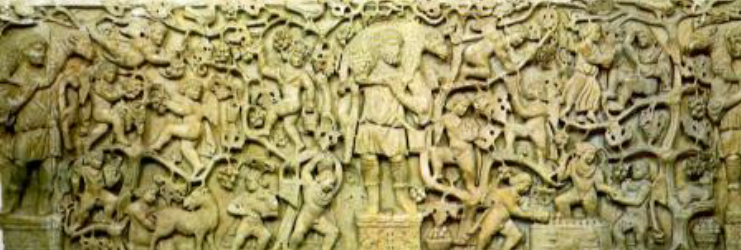
\includegraphics[width=1.0\linewidth]{04/jo_pasztor_szarkofag}
}

\paragraph{Jó Pásztor szarkofág}
Középen az antikból származó Jó Pásztor (= Jézus, a jóságos vezető) alakja, körülötte növényi ornamentika és állat-motívumok – értelmezés: szőlőindák, szőlőszüretelők (= bor, azaz Krisztus vére; a hit hirdetői) és keresztény állat-szimbólumok
Stílus: dekoratív (díszítő jellegű)(antik hagyomány), ugyanakkor keresztény tartalmú.

\paragraph{Passió-szarkofág}
Passió = a szarkofág-dombormű témája, Jézus szenvedése igen gyakori téma, hiszen a sokáig üldözött keresztényeket kitartásra buzdította.

Stílusa plasztikusan (magasan) faragott, a figurák kiugranak a falsíkból. A világos és sötét felületek kontrasztjai gyakoriak, itt már el vannak választva egymástól a jelenetek.

Leírás:
	\begin{compactitem}
		\item Balra: Krisztus ostorozása; Krisztus megkoronázása
		\item Jobbra: Krisztus Pilátus előtt; Pilátus a kezét mossa
		\item Középen: a feltámadt Krisztus szimbolikus ábrázolása
		\item Alul kétoldalt: a katonák, akik a zsidó főpapok kérésére őrizték a sírt (hogy Jézus hívei el ne lophassák a holttestet, és ne mondhassák azt, hogy eltűnt a test, tehát feltámadt).
		\item Felül középen: XP jel, ami Krisztus-monogram.
	\end{compactitem}

\tcbox[colback=darkgray!85!black,
left=0mm,right=0mm,top=0mm,bottom=0mm,boxsep=1mm,toptitle=0.5mm,bottomtitle=0.5mm,
title=\centering{Passió szarkofág dombormű}]{
	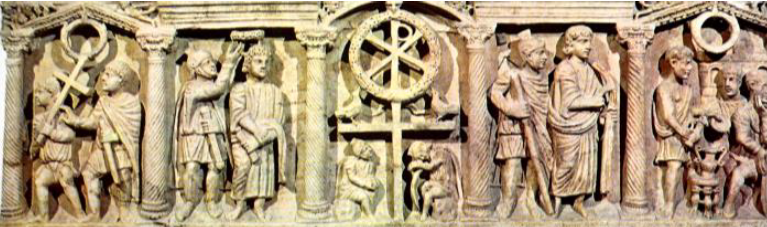
\includegraphics[width=1.0\linewidth]{04/passio_szarkofag}
}

\clearpage

\subsection*{Bizánci művészet}

\subsubsection{Építészet}

	\paragraph{Kosárfejezet}
	A bizánci építészet jellemző fejezet típusa: az ún. kosárfejezet. Sűrű indadísz, kosárhoz hasonló motívumot hoz létre. Áttört a fejezet.
	
	\paragraph{Csegelyes kupola}
	a bizánci építészetre jellemző boltozat, amikor a kör alaprajzú kupola súlyát ún. csegelyek, azaz ívháromszögek vezetik le a négyzet alaprajzú tér sarkain álló pillérekre.
	
	\begin{figure}[H]
		\centering
		\begin{minipage}{0.45\textwidth}
			\tcbox[colback=darkgray!85!black,
			left=0mm,right=0mm,top=0mm,bottom=0mm,boxsep=1mm,toptitle=0.5mm,bottomtitle=0.5mm,
			title=\centering{Kosárfejezet}]{
				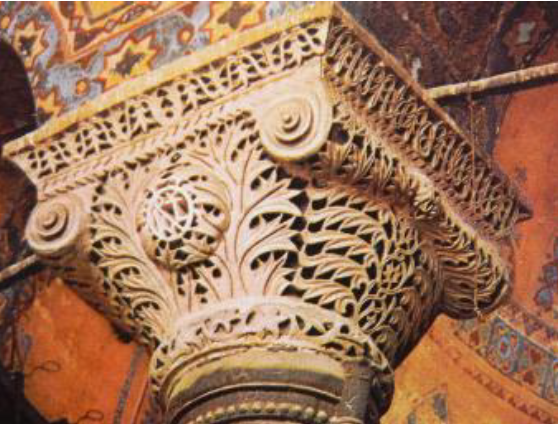
\includegraphics[width=1.0\linewidth]{04/kosarfejezet}
			}
		\end{minipage}
		\hfill
		\begin{minipage}{0.42\textwidth}
			
			\tcbox[colback=darkgray!85!black,
			left=0mm,right=0mm,top=0mm,bottom=0mm,boxsep=1mm,toptitle=0.5mm,bottomtitle=0.5mm,
			title=\centering{Csegelyes kupola}]{
				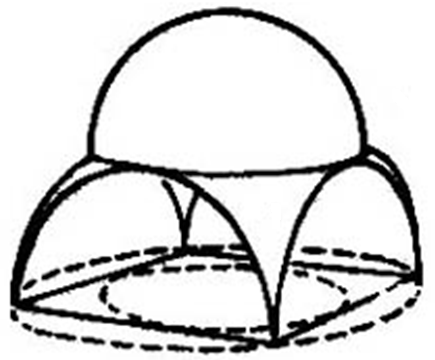
\includegraphics[width=1.0\linewidth]{04/csegelyes_kupola}
			}
		\end{minipage}
	\end{figure}
	
	\paragraph{Alaprajz}
	Ötvöződik a centrális és a longitudinális (hosszanti) térelrendeződés.
	
	\tcbox[colback=darkgray!85!black,
	left=0mm,right=0mm,top=0mm,bottom=0mm,boxsep=1mm,toptitle=0.5mm,bottomtitle=0.5mm,
	title=\centering{Hagia Sophia, Kostantinápoly}]{
		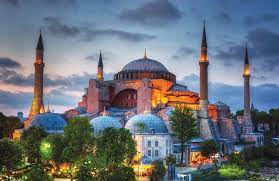
\includegraphics[width=0.54\linewidth]{04/hagia_sophia}
		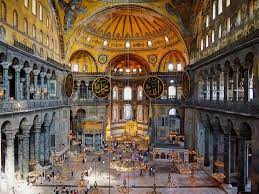
\includegraphics[width=0.46\linewidth]{04/hagia_sophia_belseje}
	}

	\paragraph{Hagia Sophia, Konstantinápoly}
	Alaprajzában ötvöződik a centrális és a longitudinális (hosszanti) térelrendeződés, ami a bizánci építészet legfőbb jellemzője.
	
	Centrális elrendezésre jellemző vonásai a középponti kupola, és az épület négyzet alakú alapja.
	
	Hosszanti (longitudinális) elrendezésre utal hosszúkás főhajója, két mellékhajóval, illetve a bejárattól a szentélyig vezető szent út. Az épület további terekkel többszörösen bővített.
	
	Eredetileg keresztény templom volt, ma török dzsámiként működik. Minaretekkel egészítették ki.
	
	A kupola hatalmas tömege kapja a főszerepet, a mellékterek egyre alacsonyabbak.
	
	Belső terének jellegzetessége a bizánci templomépítészetre jellemző kosérfejezet és csegelyes kupola.

\vspace{0.5cm}

\tcbox[colback=darkgray!85!black,
left=0mm,right=0mm,top=0mm,bottom=0mm,boxsep=1mm,toptitle=0.5mm,bottomtitle=0.5mm,
title=\centering{San Vitale, Ravenna}]{
	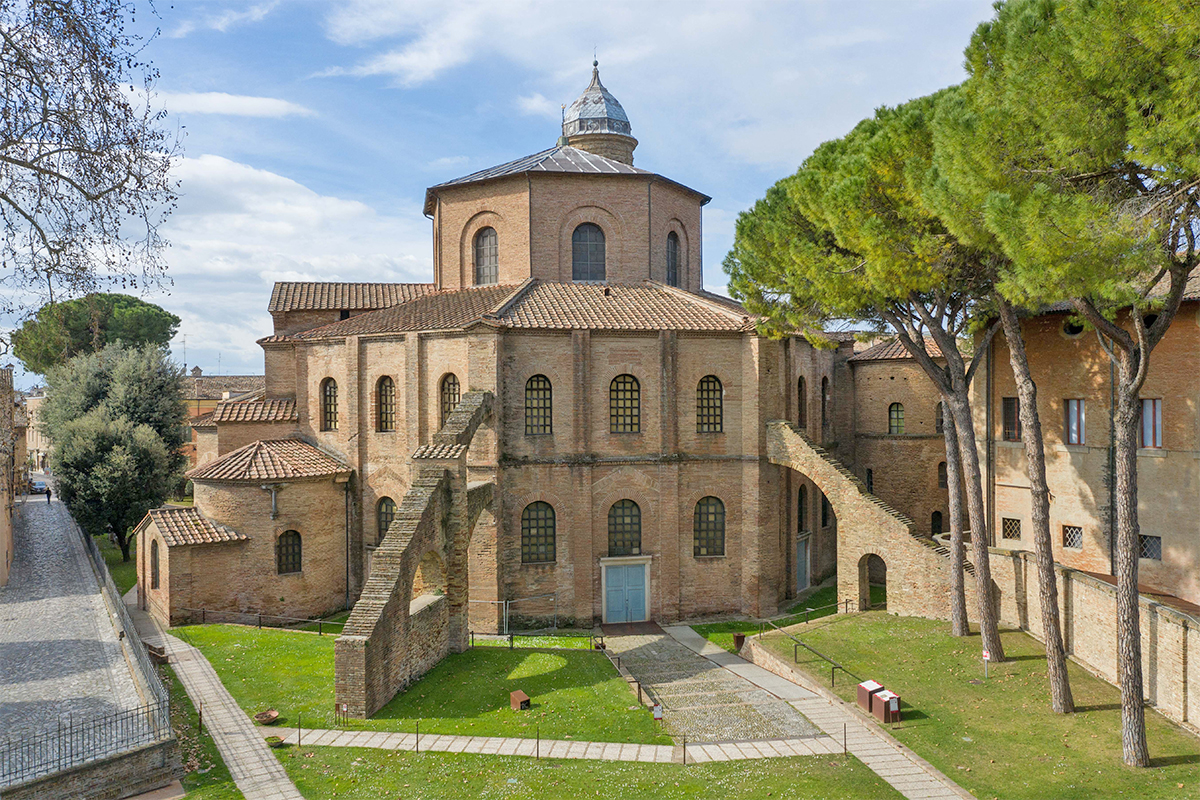
\includegraphics[width=0.54\linewidth]{04/san_vitale}
	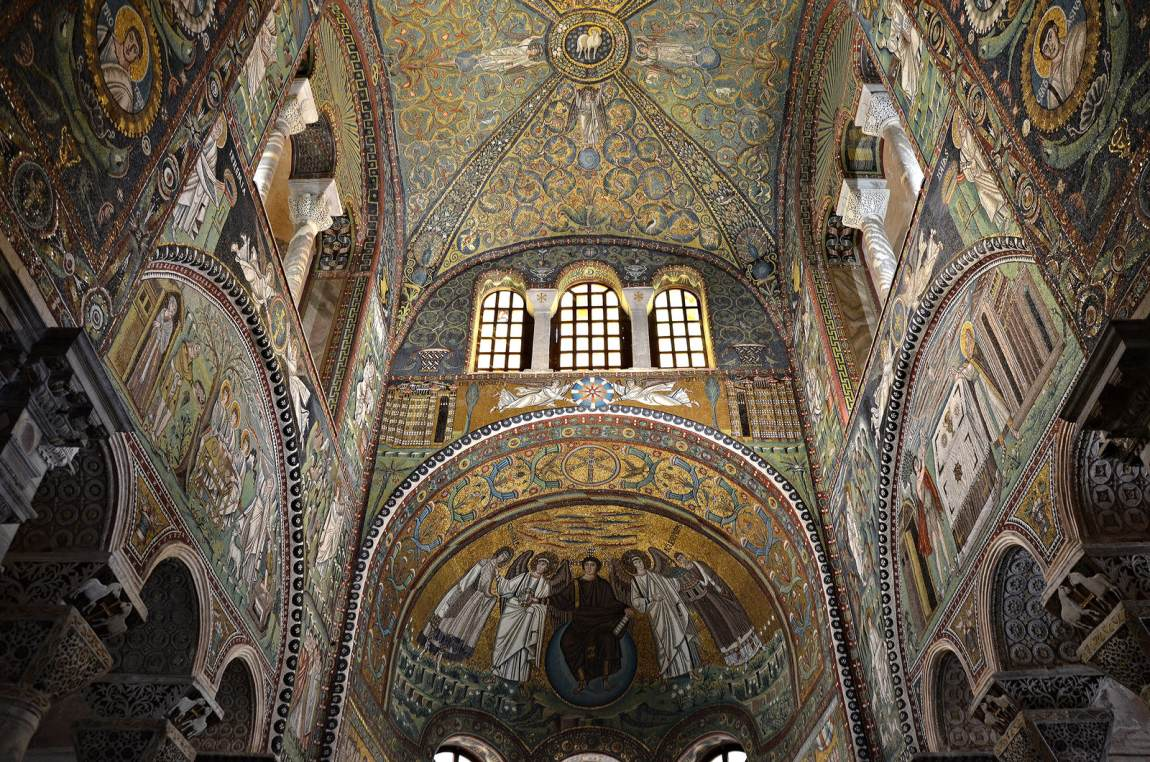
\includegraphics[width=0.46\linewidth]{04/san_vitale_belseje}
}

\paragraph{San Vitale, Ravenna (Itália)}
Justinianus császár építtette, a VI. században fejezték be.

Alaparajzában a centrális jelleg kapja a fő hangsúlyt. Nyolcszöges belső tere kupolával fedett. A nyolcszög körül alacsonyabb körüljáró található. Keleten egy félköríves apszis kapcsolódik, mellette egy-egy kiszolgáló helység kapcsolódik. Nyugaton narthex kapcsolódik hozzá.

Belsejében a nyolcszögek sarkain erős pillérek vannak. A pillérek között hármas árkádok
vannak két oszlopon. Felső szinten galéria található, ami szintén hármas
árkádokkal nyílik a belsőbe. Legfelül a kupola kiemelkedő falterületén
ablaknyílások vannak.

Külseje az ókeresztény épületekhez hasonlóan puritán, díszítetlen.
	
\subsubsection{Ikonfestészet}

\paragraph{Jelentése}
Eikon, jelentése: kép
Fatáblára festett vallásos tárgyú kép. A V. században az ókeresztény és kora bizánci korban alakult ki, virágkorát a középkor idején éli Görögország területein és Oroszországban, tehát azokon a vidékeken, ahol az ortodox, azaz görögkeleti egyház él.

\paragraph{Hagyománya}
Az ikonok rendkívül hasonlítanak egymáshoz, szinte egy sémára készülnek. Ennek oka az, hogy az ikonfestők nem egy önálló mű létrehozására törekedtek, hanem a legelső ikonokat akarták konzerválni, úgy, hogy mindig az előző képet másolták. Mindezt pedig azért tették, mert úgy tartották, hogy az első ikonképeket nem emberi kéz, hanem angyalok vagy az első szentek készítették.

\paragraph{Szigorú szabályok}
A 797-es zsinat megszigorította az ikonfestést, hogy a tárgy bálványozását megakadályozza: szabályokba foglalta, hogy kit hogyan kell ábrázolni, egy témának mik az ábrázolási szabályai, az ikonoknak milyen lehet a stílusuk, és pontról pontra azt is, hogy az ikont hogyan kell elkészíteni.

\paragraph{Stílus}
Nincsen térmélység. A háttérben általában arany szín jelenik meg.
A figurák életszerűtlenek, a mozdulatok merevek. Az arcok
síkszerűek, a drapéria redői vonalakkal, rajzosan előadottak.
Az arc kifejezése általában komor, szomorkás. A színek általában
szimbolikusak, az arany a természetfölöttiséget, a fekete a gyászt,
a bíbor a dicsőséget jeleníti meg. A gyermek Jézus ábrázolásánál
a gyermek arányai egy felnőtt arányait tükrözik. Az ikonok nagyon
hasonlítanak egymásra, egyfajta sematizmus jellemzi őket.

\paragraph{Fő témái}

	
	\begin{figure}[H]
		\centering
		\begin{minipage}{0.2\textwidth}
			\tcbox[colback=darkgray!85!black,
			left=0mm,right=0mm,top=0mm,bottom=0mm,boxsep=1mm,toptitle=0.5mm,bottomtitle=0.5mm,
			title=\centering{Eleusza}]{
				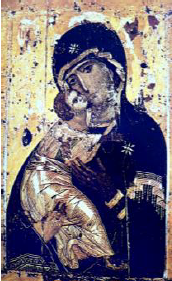
\includegraphics[width=1.0\linewidth]{04/eleusza}
			}
		\end{minipage}
		\hfill
		\begin{minipage}{0.22\textwidth}
			
			\tcbox[colback=darkgray!85!black,
			left=0mm,right=0mm,top=0mm,bottom=0mm,boxsep=1mm,toptitle=0.5mm,bottomtitle=0.5mm,
			title=\centering{Útmutató Madonna}]{
				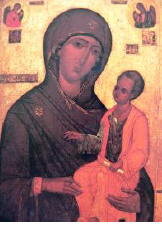
\includegraphics[width=1.0\linewidth]{04/utmutato_madonna}
			}
		\end{minipage}
		\hfill
		\begin{minipage}{0.25\textwidth}
			
			\tcbox[colback=darkgray!85!black,
			left=0mm,right=0mm,top=0mm,bottom=0mm,boxsep=1mm,toptitle=0.5mm,bottomtitle=0.5mm,
			title=\centering{Pantokrátor}]{
				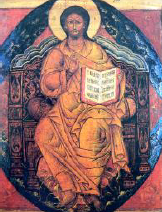
\includegraphics[width=1.0\linewidth]{04/pantokrator}
			}
		\end{minipage}
		\hfill
		\begin{minipage}{0.22\textwidth}
			
			\tcbox[colback=darkgray!85!black,
			left=0mm,right=0mm,top=0mm,bottom=0mm,boxsep=1mm,toptitle=0.5mm,bottomtitle=0.5mm,
			title=\centering{Hagiographikus}]{
				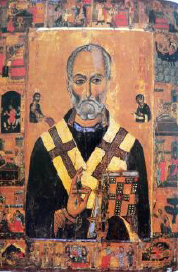
\includegraphics[width=1.0\linewidth]{04/hagiographikus}
			}
		\end{minipage}
	\end{figure}
	

	\subparagraph{Eleusza}
	Az egyik leggyakoribb ikon típus. Máriát ábrázolja a gyermek Jézussal. A hagyomány szerint abban a pillanatban, amikor Jézus anyjának fülébe súgja szenvedésének történetét és halálát. A gyermek felnőttes arányai, kopaszodó homloka arra a szomorú bölcsességre utal, hogy már csecsemőként tisztában van sorsával. Mária csüggedő arckifejezése és fekete ruhája a gyászt, a bánatot tükrözi.
	
	\subparagraph{Útmutató Madonna}
	Mária a gyermekre mutat, mintha azt mondaná: „Őt kövessétek!”. A gyermek a nézők felé fordulva megáldja őket.
	
	\subparagraph{Pantokrátor}
	Nagyon gyakori téma, amikor Krisztus a világ uraként trónuson ül, teste körül dicsfény vagy más értelmezés szerint a világ gömbje van. Az arca szigorú. Baljában könyv, ez a tanítására utal, ha a könyv csukott, már számon kéri tanítását. Jobb kezével áldó mozdulatot tesz.
	
	\subparagraph{Hagiographikus ikon}
	Olyan ikontípus, ahol a szent középen, frontálisan ábrázolt, körülötte pedig
	életének jelenetei vannak kis képekben előadva.

\clearpage
	
\subsubsection{Mozaikművészet}

	Bizáncban a császár nem csak a politikai hatalom képviselője volt, hanem egy személyben az egyház feje is, hatalmtár Isten kegyelméből valónak tartotta. Ezt az államformát cezaropapizmusnak nevezik (császárpápaság).
	
	\paragraph{Jusztiniánusz császár és kísérete}
	A mozaik a San Vitale szentélyben található a szentélyfalon.
	
	\tcbox[colback=darkgray!85!black,
	left=0mm,right=0mm,top=0mm,bottom=0mm,boxsep=1mm,toptitle=0.5mm,bottomtitle=0.5mm,
	title=\centering{Jusztinianusz császár és kísérete mozaik, San Vitale, Ravenna}]{
		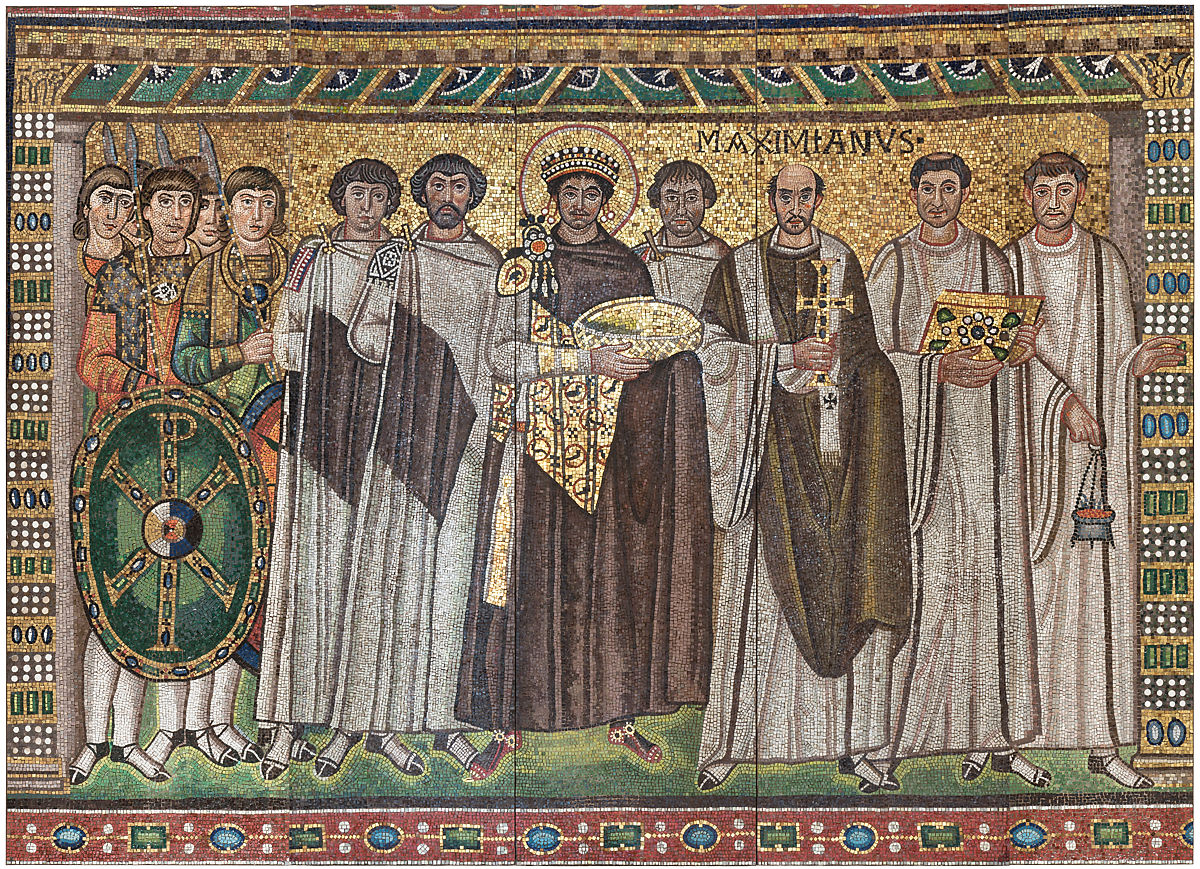
\includegraphics[width=1.0\linewidth]{04/jusztinianusz}
	}
	
	\subparagraph{Leírás}
	\begin{compactitem}
		\item Középen Jusztiniánusz császár, kezében liturgikus tál, amiben az oltáriszentséget, a szentostyát tartják
		\item balra magas rangú kísérői: fő politikusai, a politikai hatalom birtokosai
		\item balszélen katonák, a hatalom biztosítói, pajzsukon az XP-monogrammal
		\item jobbra Ravenna püspöke, a vallási hatalom birtokosa (felette a neve: Maximianus)
		\item jobbra további főpapok, kezükben liturgikus tárgyakkal
	\end{compactitem}

	\subparagraph{Stílusa}
	\begin{compactitem}
		\item nem reális-földi térben állnak az alakok, mögöttük arany háttér
		\item nincs térmélység: a figurák egymás lábán „taposnak”, azonos magasságúak
		\item a testtartások merevek, a figurák frontális beállításúak
		\item a drapériák függőleges redői monotonon sorolódnak egymás mellé (ritmus)
		\item az arcok egyformák, kifejezéstelenek, a tekintetek merevek, megközelíthetetlenséget sugallnak
	\end{compactitem}

	\subparagraph{Értelmezés}
	A császár a politikai és a vallási hatalom képviselőivel együtt jelenik meg, ő a politikai és a vallási hatalom vezetője egy személyben, azaz hatalmát Istentől eredezteti (feje körül glória is van) = cezaropapizmus (császárpápaság); államában politika és vallás egyenrangú.
	
	

\subsubsection{Szobrászat}

\begin{wrapfigure}{r}{0.2\textwidth}
	\tcbox[colback=darkgray!85!black,
	left=0mm,right=0mm,top=0mm,bottom=0mm,boxsep=1mm,toptitle=0.5mm,bottomtitle=0.5mm,
	title=\centering{Diptichon}]{
		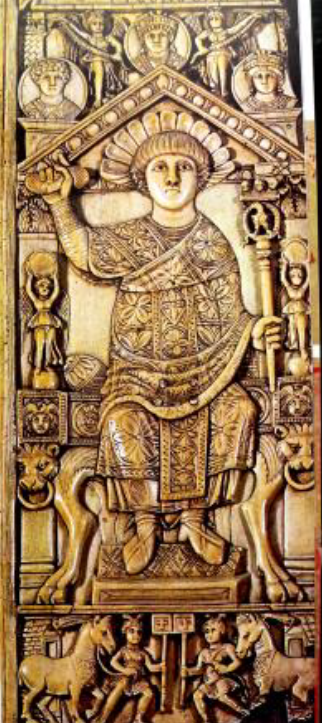
\includegraphics[width=1.0\linewidth]{04/diptichon}
	}
\end{wrapfigure}

A bizánci szobrászatban sem jellemzőek az épületeket díszítő nagyméretű körszobrok: általában kisméretű, elefántcsontból készült, laposan faragott tárgyak, ún. konzuli dipitichonok (= két részből álló, könyvszerűen összecsukható tárgy; a bizánci császár ajándékozta legfőbb politikusainak kinevezésük alkalmából) maradtak fenn a korból.

A diptichonok stílusában a bizánci mozaikok stílusa ismétlődik: frontálisan ábrázolt, merev tartású, kifejezéstelen arcú figura, akinek alakja trónuson ülve hatalmat, tekintélyt fejez ki.

\cleardoublepage

\section{Az ikonfestészet}

\begin{center}
	\begin{longtable}{ | p{0.25\textwidth} | p{0.75\textwidth} | }
		
		\hline
		\multicolumn{2}{|c|}{\textbf{A tétel adatai}}
		\\ \hline
		
		\hline
		Tétel teljes címe 
		&
		Milyen szabályrendszer határozza meg az ikonok képi világát? Mutassa be az ikonfestés technikáját, lépéseit! Milyen anyagok szükségesek egy ikon festéséhez? Milyen eszközök szükségesek az aranyozáshoz?
		\\ \hline
		
	\end{longtable}
\end{center}

\subsection*{Rendeltetése}

Az ikon görög eredetű szó, ikóna, jelentése: „kép“, „képmás“. Ikonokon elsősorban a keleti egyházak szentképeit értjük, különösen az ortodox egyház és az abból kivált és Rómával egyesült, bizánci rítusú görög katolikus egyház liturgikus képeit. Ezek a képek általában fel vannak szentelve, és a keleti egyházak teológiájában valamint spiritualitásában rendkívüli szerepet játszanak.

Az ikonok célja Isten és szentjei tiszteletének tudatosítása, valamint az ábrázolt személy és a szentkép előtt imádkozó személy közötti kapcsolatteremtés, így tehát átvitten a vallásos szemlélődő és Isten közötti kapcsolat megteremtése.

Az ikonokat ennek megfelelően a keleti egyházakban nem tartják sem műtárgynak, sem dekorációnak.

Az ikon festmények nem műtárgyak. Az ikonfestészet alkotásai nem a dekorációt szolgálják. Megszentelt képek, melyek célja az Isten és az ember közötti kapcsolat kialakítása. A nyugat-európai szentkép realisztikusan ábrázolja témáját. Az ikonnál azt érezzük, hogy meditációt közvetít.

\subsection*{Mi az ikon?}

Az ikonok háttere általában aranyszínű, és a lerajzolt szent szembenéz velünk. Bizáncban azonban Krisztus (Megváltó), Mária (Istenszülő), a szentek, mártírok, angyalok és a Szentírás történeteinek képi ábrázolásait jelentette. Kezdetben ikon alatt nem csupán a napjainkban használatos fatáblára festett szentképeket értették, hanem a szobrokat, domborműveket is ezzel a szóval jelölték. \textbf{Ma ikon alatt önálló, hordozható (azaz nem épületek falára készített) festményt, mozaikot értünk}, ezen belül is \textbf{szentkép}et, s a továbbiakban is ebben az értelmében használjuk ezt a fogalmat. Az ikonok \textbf{az ortodox egyház szentképei}.

\subsection*{Története}

A keleti ortodox hagyomány szerint az ikonfestészet megteremtése már a kereszténység nagyon korai szakaszában elkezdődött Európában. A 10. század végétől Oroszországban is elterjedt a kereszténység. Ezzel egy időben az ikonfestészet is kezdetét vette. Az ikon szerves része lett nemcsak az orosz kultúrának, hanem a középkori Európának is. A bizánci ikonfestészet a képrombolás korát (726-843) követően virágzott először, bár már a kora bizánci, Jusztiniánusz-kori művészetben is, sőt a képrombolás ideje alatt is készültek ikonok, valamint ekkor (az 5-7. században) alakultak ki a később is jelentős festőiskolák, festészeti központok (Konstantinápoly, Thesszaloniki, Ravenna, Alexandria, továbbá a kopt és szíriai iskolák).

\subsection*{Szabályai}

Az ikonfestés évszázados hagyományokra tekint vissza. Az ikon tulajdonképpen fára festett kép. Korábban ikont csak szerzetesek festettek, a képek mély imádságból születtek.

Az ikonfestés szabályai szigorúak, pontosan meghatározott, hogy egyes témákban az adott személyt, ünnepet milyen forma, illetve szimbolika jellemezze. A kritériumoknak eleget téve egyéni stílusok is kialakultak. Évszázadok óta alig változott festés technikája és tartalma, amit írásba is fektettek, szentesítettek és szabályoztak.

Az ikonfestő, technikai kivitelező, aki az ikont nem kitalálja, hanem az egyház törvénye és hagyománya alapján létrehozza a szentatyák által meghatározott normák és kompozíciók szerint.

Az ikon festmények meghatározott színvilágot hordoznak. Az ikonon minden színnek saját jelentése van. Ezért Krisztus, Szűz Mária és a szentek ruháit vagy azok részeit, esetleg a fej körüli glóriát arannyal festették. A kör, mint a legegyszerűbb és legtökéletesebb forma egy másik módja annak, hogy kijelölje az eget, ellentétben a Földet szimbolizáló térrel. Az aranyszínű elömlő fény, a zöld, a fényes okker, a rózsaszín és az ibolya finom árnyalatai, valamint a kék égbolt az ősi szépség, a mennyei harmónia képe.

A védelem érdekében néhány ikonhoz külön fedélféle tartozik. Arany vagy ezüstborításúak, drágakövekkel díszítettek. Ezek a bizánci művészetből származnak. A kor uralkodói és nemesei a legjobb ékszerészektől rendelték a külső borítást.



\begin{wrapfigure}{r}{0.45\textwidth}
	\tcbox[colback=darkgray!85!black,
	left=0mm,right=0mm,top=0mm,bottom=0mm,boxsep=1mm,toptitle=0.5mm,bottomtitle=0.5mm,
	title=\centering{Andrej Rubljov: Angyali üdvözlet ikon}]{
		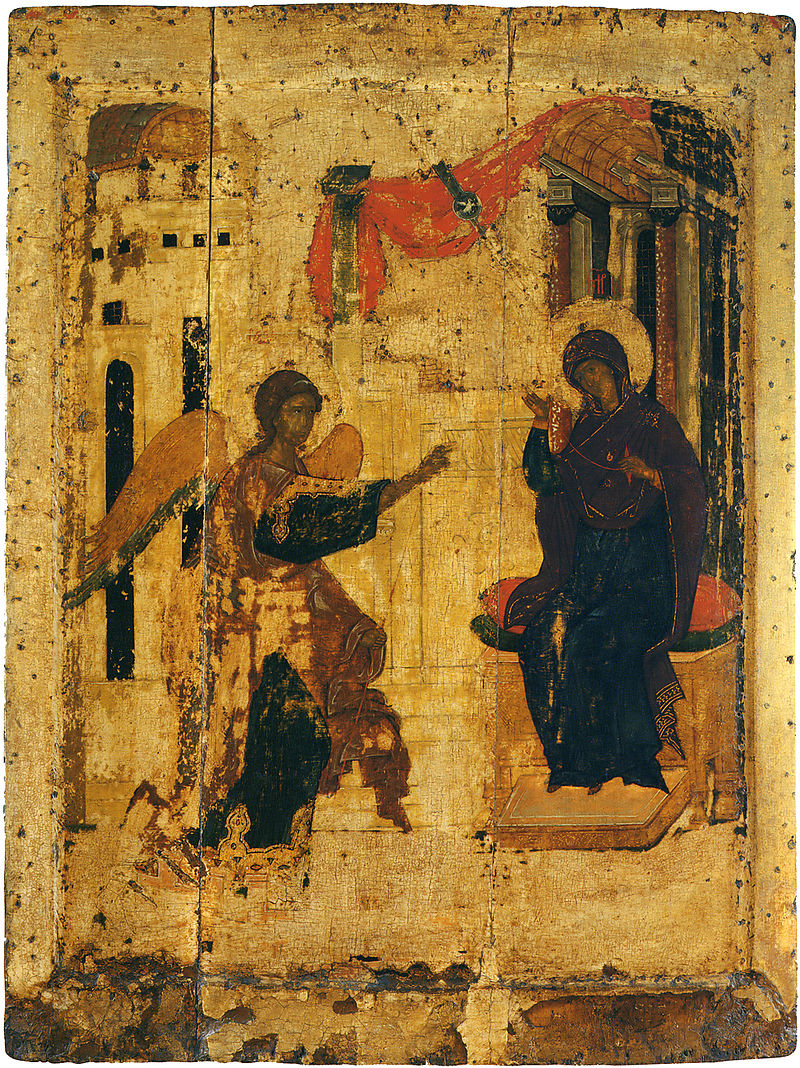
\includegraphics[width=1.0\linewidth]{04/angyali_udvozlet}
	}
\end{wrapfigure}

Az ikon megalkotása nem rutin és technikai tudás kérdése. A tehetség kevés hozzá, mert alázatosság és hit nélkül a festő nem tudja elkészíteni. Az ikon festmények spirituális tanítása elsősorban azt üzeni, hogy az ikonfestés szolgálat. A festő nem is írja alá művét, hiszen ő csak közvetítő, az alkotás az Úré. A festő névtelen maradt, nem lépett be az ikon megszentelt terébe. Az ikon Istennel való élő kapcsolat, Isten megismerésének az eszköze. Szimbolikusan a beállítás ugyanolyan szerepet játszott, mint az arany háttér: Isten világának világosságát és szépségét kívánta megmutatni.

Az ikonok aranyszínű háttere a szellemi világ és az isteni sugárzás szimbóluma. Az ikonok – fára rajzolt, aranyozott szentképek – központi szerepet foglalják el az ortodox egyházban, és a katolikus egyházban is elterjedt volt egészen a XIII. századig (és helyenként ma is használják). Az ikon a keresztény egyházban az Isten megismerésének egyik eszköze, és éppen ezért monumentálisnak és lenyűgözőnek kell lennie.

Annak ellenére, hogy az ikonfestők nagyon szigorú szabályok, az egyház által lefektetett kánon által kell, hogy dolgozzanak, a művészet más formában tudott megnyilvánulni: az egyházi kánonok szükségszerűsége egy keretet adott az ikonnak, maga a festő pedig arra tudott koncentrálni, hogy az ikonnak lelket adjon, minél közelebb hozza azt az emberhez. Ez pontosan megnyilvánult az egyik leghíresebb ikonfestő, Andrej Rubljov (1360-1428) alkotásaiból, akik képeinek kifejezett egyéniséget és orosz vonásokat tudott adni. Magát az ikonfestő mestert azonban régen nem tartották az ikon szigorúan vett szerzőjének: úgy gondolták, hogy a szent ikont maga az Isten rajzolja meg az adott mesteren keresztül.

Ha az ikon eseményeket ábrázol, akkor nem kell törekednünk az események sorrendjének és idejének a megfejtésére, éppen amiatt, hogy időbeli tényező itt nem érvényesül.

\subsection*{Jellemzői}

\begin{wrapfigure}{r}{0.45\textwidth}
	\tcbox[colback=darkgray!85!black,
	left=0mm,right=0mm,top=0mm,bottom=0mm,boxsep=1mm,toptitle=0.5mm,bottomtitle=0.5mm,
	title=\centering{Fordított perspektíva}]{
		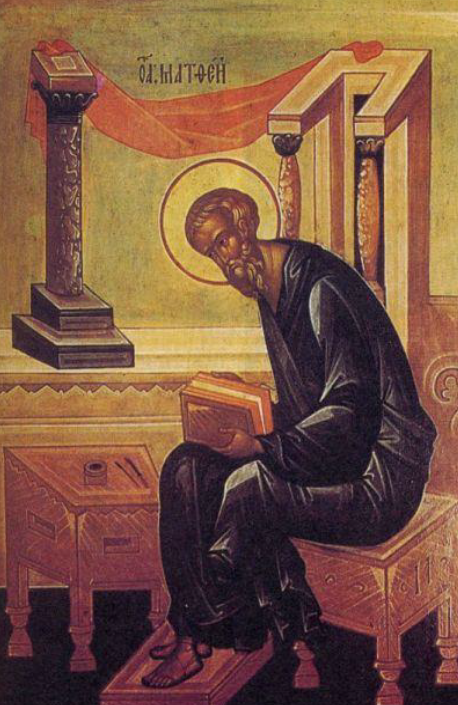
\includegraphics[width=1.0\linewidth]{04/forditott_perspektiva}
	}
\end{wrapfigure}

\paragraph{Fordított perspektíva}
Lényege, hogy eltűnő pontjai a festményen kívül helyezkednek el. Így azt a látszatot keltik, hogy ezek a pontok a kép előtt vannak. Ezáltal a kép egy ablak lesz, melyen át az égi világba pillanthat a néző.

Az ikonoknak nincs linearitása és nincs időbelisége sem: az egyházi tanítás szerint Isten mindenhol jelen levő és Isten örökkévaló. Ebből kiindulva az ikon egyszerre több nézőpontból mutatja be a képet, és úgy nevezett fordított perspektíva érvényesül.

Tehát vonalai a perspektívával szemben nem össze ("a párhuzamosok a végtelenben találkoznak"), hanem szét tartanak.

\paragraph{Mintakönyvek}

Ezekben volt pontosan leírva az ikonok festésének szigorú szabályai, mintái amelyek alapján a mesterek dolgoztak.

\paragraph{Fatábla használata}
A régi ikonfestő minidig fatáblát használt az ábrázolás hordozójaként. Teológiai okai voltak, amiért a fát részesítették elényben a vászonnal szemben. Míg a vászon mozog, szinte lebeg, addig a fatábla alig változik, a változatlanság, az örökkévalóság érzetét kelti.

\subsection*{Eljárás}
\begin{enumerate}
	\item A faléceket egymás mellé illesztik. Hátulról egy heveder léccel rögzítik.
	\item A festendő felületet állati enyvvel kenik be.
	\item Fehérvásznat feszítenek ki a festendő felületre és alapozzák. (fehér vászon utal Veronika kendőjére vagy Krisztus halotti leplére, mely leplek a hagyomány szerint az első Krisztus-képmást őrizték meg)
	\item Először a körvonalakat rajzolják meg.
	\item Fölteszik az aranyat.
	\item Festés (kifestés), sötét színektől a világos színek felé haladnak
	\item Gyakran fémborítást helyeznek az alakon kívüli részekre.
\end{enumerate}

\subsection*{Aranyozás}

\subsubsection{Eszközei}

\begin{itemize}
	\item aranyozó párna (kb. 25 x 15 cm nagyságú borjúbőrrel bevont alápárnázott kőrisfadeszka),
	\item aranyozó kés, 
	\item mókusfarok, alsó végén hajecsettel,
	\item kétvégű kis hajecset,
	\item libbentő (ansieszer),
	\item besöprő ecsetek,
	\item achát kő.
\end{itemize}

\begin{figure}[H]
	\centering
	\begin{minipage}{0.23\textwidth}
		\tcbox[colback=darkgray!85!black,
		left=0mm,right=0mm,top=0mm,bottom=0mm,boxsep=1mm,toptitle=0.5mm,bottomtitle=0.5mm,
		title=\centering{Füstarany}]{
			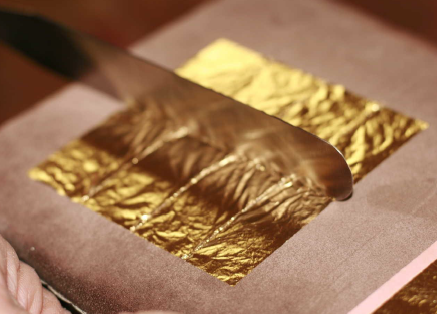
\includegraphics[width=1.0\linewidth]{04/aranyfust}
		}
	\end{minipage}
	\hfill
	\begin{minipage}{0.23\textwidth}
		
		\tcbox[colback=darkgray!85!black,
		left=0mm,right=0mm,top=0mm,bottom=0mm,boxsep=1mm,toptitle=0.5mm,bottomtitle=0.5mm,
		title=\centering{Besöprő ecset}]{
			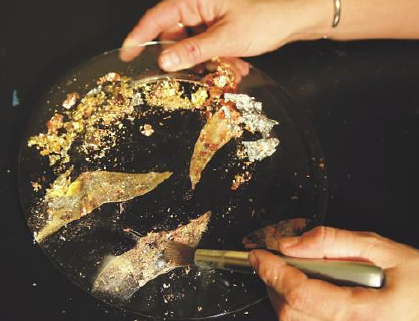
\includegraphics[width=1.0\linewidth]{04/ecset}
		}
	\end{minipage}
	\hfill
	\begin{minipage}{0.23\textwidth}
		
		\tcbox[colback=darkgray!85!black,
		left=0mm,right=0mm,top=0mm,bottom=0mm,boxsep=1mm,toptitle=0.5mm,bottomtitle=0.5mm,
		title=\centering{Kés és párna}]{
			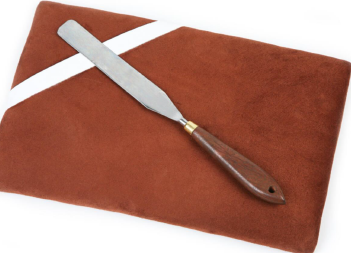
\includegraphics[width=1.0\linewidth]{04/kes_parna}
		}
	\end{minipage}
	\hfill
	\begin{minipage}{0.21\textwidth}
		
		\tcbox[colback=darkgray!85!black,
		left=0mm,right=0mm,top=0mm,bottom=0mm,boxsep=1mm,toptitle=0.5mm,bottomtitle=0.5mm,
		title=\centering{Achát polírkő}]{
			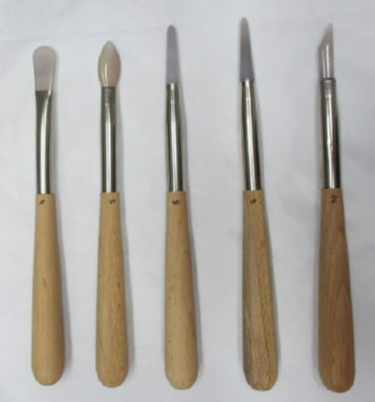
\includegraphics[width=1.0\linewidth]{04/polirko}
		}
	\end{minipage}
\end{figure}


\subsubsection{Eljárás}

\begin{enumerate}
	\item A felületet alapozom, erre jön a mixtion, amely tulajdonképpen egy ragasztóanyag. 
	\item Ha ez eléri a 99 százalékos szárazságot, akkor rárakhatom a laparanyat.
	\item Az aranyat mindig szarvasbőr párnán, úgynevezett aranyozókéssel vágom olyan darabokra, amekkorára szükségem van. Ezeket mókusszőr ecsettel teszem rá az aranyozandó felületre. 
	\item Utána hagyom száradni, majd áttörlöm.
	\item A 24 karátos aranylapokat száradás után egy féldrágakővel, acháttal is át kell polírozni, ettől lesz fényes a matt felület.
\end{enumerate}

